\chapter{Diseño e implementación del servidor}

En este capítulo se explicara el diseño y la implementación del server. En la Fig. \ref{fig:server-final} se observa la versión final del servicio, mostrando la interacción entre los Clientes, los sistemas SL y el Server.

\begin{figure}
    \centering
    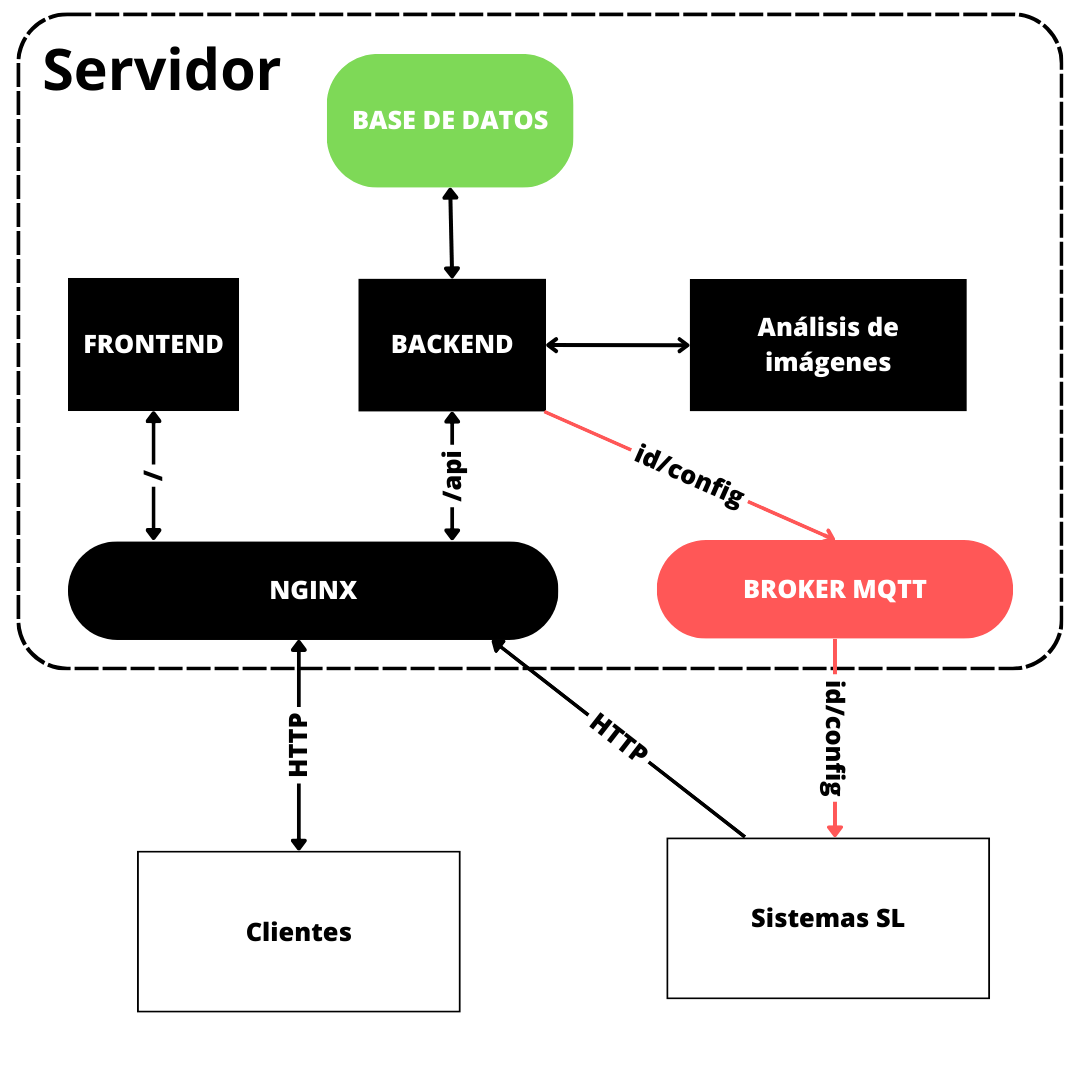
\includegraphics[width=\textwidth]{imgs/server-esquema.png}
    \caption{Esquema final del servidor.}
    \label{fig:server-final}
\end{figure}

\section{Actualidad del desarrollo web}

En la web existen dos grandes mundos, el Frontend el cual es la parte de la web con la que interactuan los usuarios o clientes. Otra parte fundamental es el Backend que es la parte que se conecta con la base de datos y ejecuta las validaciones necesarias para leer o escribir información. En general, el frontend y el backend suelen ser 2 proyectos separados y pueden ser construidos en diferentes lenguajes. Los lenguajes más utilizados son: JavaScript (JS), Python, Ruby, entre otros \cite{presta_10_2021}.

En la actualidad el formato más utilizado para trasmitir información entre el Backend y el Frontend es JSON de sus siglas en inglés JavaScript Object Notation o traducido como notación de objetos de JavaScript. En la Fig. \ref{fig:ejemplo-json} se observa un ejemplo de JSON este tipo de notación se caracteriza por almacenar los datos en forma clave-valor, permitiendo que la busqueda de información sea facil.

\begin{figure}
    \centering
    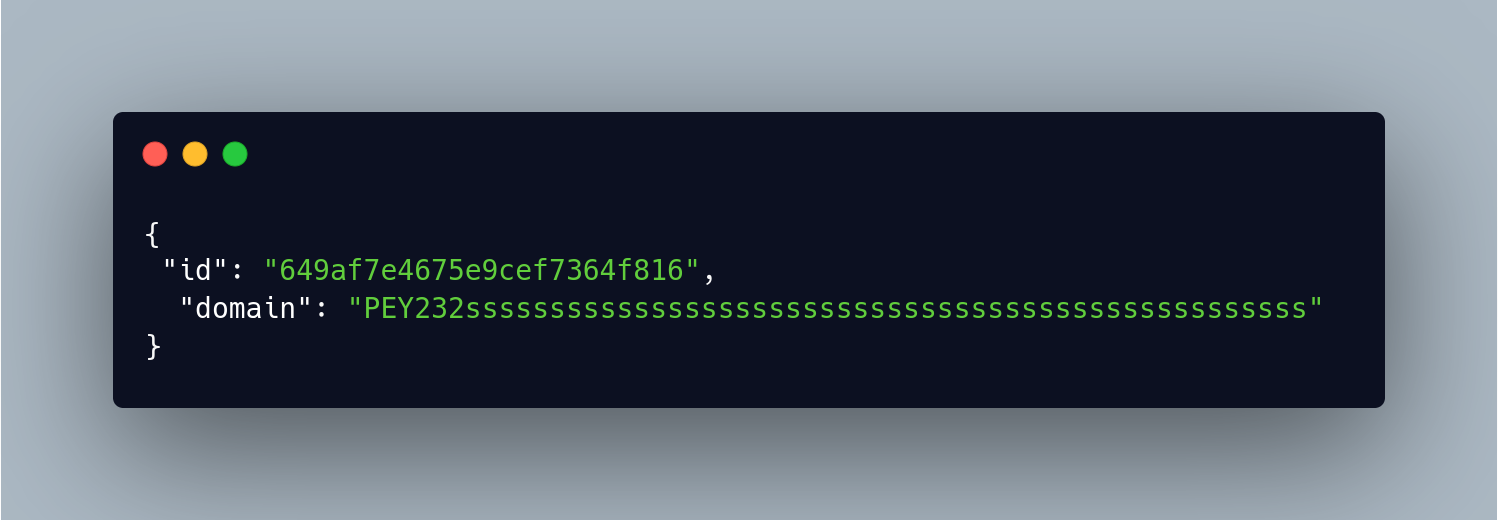
\includegraphics[width=.5\textwidth]{imgs/json-example.png}
    \caption{Ejemplificación de un JSON.}
    \label{fig:ejemplo-json}
\end{figure}

Hoy en día la web se ha transformado en la base de cualquier organización, hace años las organizaciones solían usar aplicaciones de escritorio, pero en la actualidad las aplicaciones web han ganado el mercado.

\section{Docker}


Docker es una tecnología open source desarrollada por Docker Inc, la cual permite correr aplicaciones de forma aislada en contenedores.

\subsection{¿Qué es un contenedor?}

Un contenedor funciona casi como una máquina virtual, pero sin entorno gráfico y compartiendo el Kernel \cite{keepcoding_que_2022} con el sistema que lo hospeda, lo que hace que los contenedores sean más livianos y mucho más rápidos que una máquina virtual, ya que estas últimas emulan todo el sistema e incluyen un puente entren el kernel del sistema padre y el sistema emulado. Por lo que cada contenedor puede suele estar especializado para cumplir una determinada tarea, a esos contenedores se los suele llamar servicios.

\subsection{Docker Compose}

Docker es una tecnología muy utilizada pero por si sola puede ejecutar un unico contenedor a la vez, es por ello que existen herramientas para la administración de multiples contenedores en simultanio. La más conocida, y muy utilizada en el mundo del desarrollo es Kubernetes [cita a kubernetes]. Debido a que el sistema no es lo suficientemente grande y no se cuenta con multiples servidores para alojar los servicios, la implementación se realizo mediante Docker Compose \cite{docker_inc_docker_2023}, el cual cumple un rol muy similar a Kubernetes, pero sin tanta complejidad extra que trae la opción de administrar multiples servidores.
\begin{figure}
    \centering
    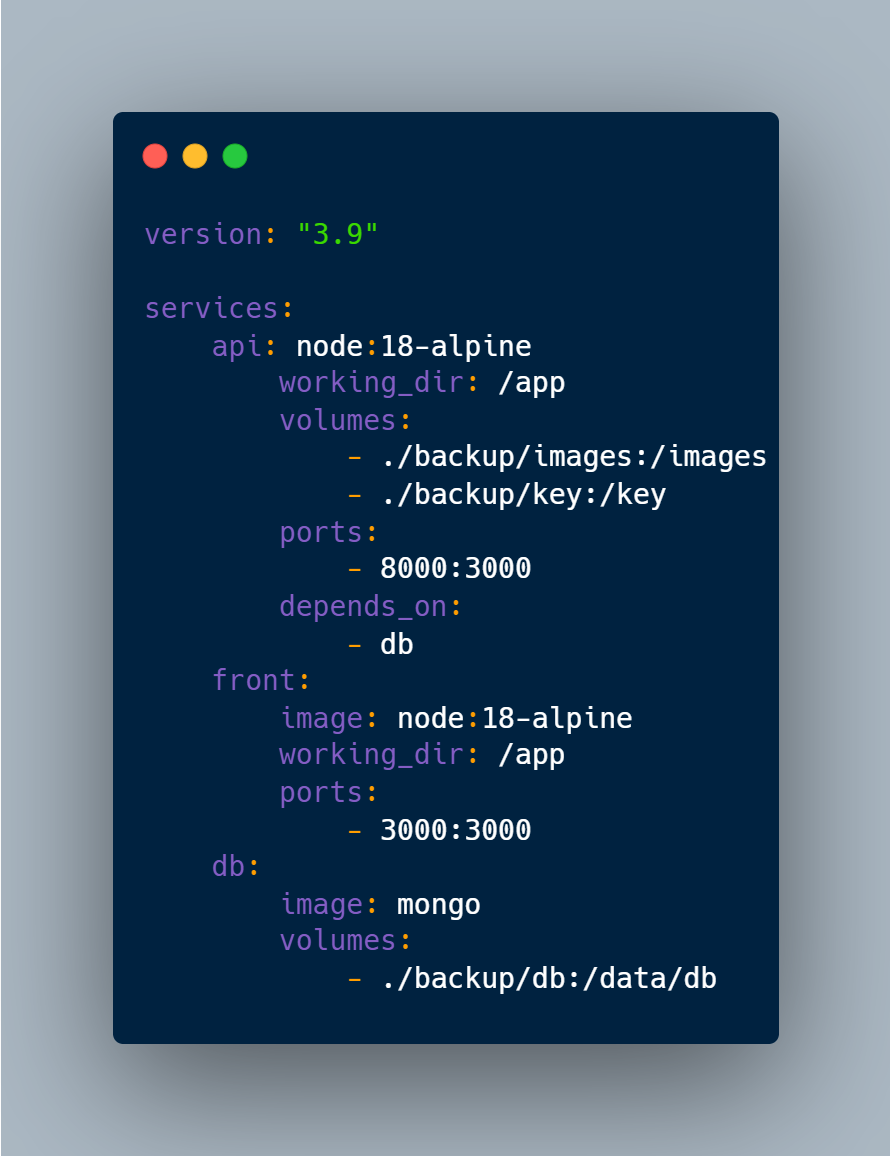
\includegraphics[width=.5\textwidth]{imgs/docker-compose.png}
    \caption{Ejemplificación de una archivo \textit{docker-compose.yml}}
    \label{fig:docker-compose-yml}
\end{figure}

El proceso de configuración de Docker compose se hace creando un archivo de extención YAML como el de la Fig. \ref{fig:docker-compose-yml}, se puede observar que existen 2 apartados principales.

\subsubsection*{version}

Este atributo le indica a Docker Compose que versión del archivo de configuración se esta utilizando, en general, esta versión impacta directamente en que atributos se pueden utilizar en el resto del archivo de configuración.

\subsubsection*{services}

Dentro del apartado de \textit{services} o por su traducción servicios se definen los servicios que se necesitaran, en este ejemplo se muestran 3 contenedores \textit{api}, \textit{front}, \textit{db}.

A su vez dentro de cada uno se define el atributo \textit{image} el cual indica que imagen se utilizara, esta imagen puede ser creada por privada o se puede utilizar alguna de Docker Hub [link docker hub] el cual es un repositorio de imagenes de Docker.
Las imagenes son en esencia un sistema operativo configurado para algunos entornos, por ejemplo la imagen \textit{node:18\-alpine} posee un sistema Alpine, que ya viene instalado con NodeJS en su versión 18, imagen muy utilizada para correr aplicación escritas en JS.
Otro campo que destaca es el \textit{working\_dir} que es el directorio de trabajo y es donde se almacenara el código de la aplicación, es importante destacar que esta ruta se toma desde el contenedor, y no tiene porque ser una ruta valida desde el sistema Host.
El atributo \textit{volumes} es un array que vincula una carpeta del sistema Host con una carpeta del contenedor, permitiendo acceder a la información del contenedor, esto es muy utilizado para realizar backup desde el sistema Host.
Por último \textit{ports} es un array que vincula los puertos del sistema anfrition a los puertos del contenedor, lo que es sumamente útil cuando se desea escuchar un puerto especifico para manejar peticiones HTTP por ejemplo.

\subsubsection*{intranet}

Docker Compose genera una red interna para interconectar los contenedores, lo que permite que el servicio \textit{api} pueda acceder a la base de datos del servicio \textit{db} mediante la ruta \textit{mongodb://db:27017/sl}. La mayor ventaja de esta red es que hace inaccesible la base de datos para usuario que no estén dentro de la red de Docker, por lo que hace menos vulnerable al sistema.

\section{Servicios}

Una vez que fue descripto como se hará la implementación y su arquitectura, se procederá a entender como fue creada la aplicación web en su totalidad, describiendo cada parte del sistema.

\subsection{Base de datos}

La base de datos elegida fue Mongo DB [documentacion de mongo], debido a que una de las bases de datos más utilizada. Mongo es una base de datos del tipo NoSQL y es basada en documentos, por lo tanto no posee vinculos fuertes entre los diferentes esquemas.
Los datos se almacenan en BSON (binary JSON), el cual hace más fácil la transferencia de datos. Por otro lado, permite escalar de forma horizontal de forma mucho más sencilla, ya que se suelen usar identificadores únicos y no incrementales, como es frecuente en bases de datos del tipo SQL.



El esquema de base de datos [figura de la base de datos].

\subsection{Broker MQTT}

Debido a que Mosquitto es el broker MQTT más utilizado, el cual utiliza la versión 5.0 del protocolo. Elúnico tópico implementado en el de configuración de las barreras, este tópico tiene la forma de ``\textit{id}/config" donde \textit{id} es el id único de la barrera, esto permite de que existan tantos tópicos como barreras, y solo pueden escuchar los cambios de configuracíón de ellas, lo que permite ahorrar procesamiento de datos en la barrera.

\subsection{Backend}

El Backend esta implementado en NestJS \cite{noauthor_documentacion_nodate}. Su principal función es la de administrar la información por que se conecta con la base de datos para realizar las tareas de lectura y escritura de documentos.

Con la idea de generar la mayor documentación posible de este servicio se utilizo una libreria llamada Swagger el cual junto a NestJS genera documentación automatica de los las rutas HTTP. Esto facilita la tarea de crear una nueva aplicación asi como la de incluir una nueva persona al proyecto. El la Fig. \ref{fig:swagger-example} se observa como se ve la documentación generada por Swagger.

Debido a la necesidad de autenticación de usuarios, y de los sistemas SL se implemento PassportJS [doc passport] la cual permite la creación de sistemas de validación de forma más sencilla. Los métodos de autenticación implementados fueron:

\begin{enumerate}
    \item Usuario y contraseña: Utilizado para los usuarios que entran/registran desde la web.
    \item ApiKey de terceros: Una forma de validar si la aplicación que pide datos está autorizada o no.
    \item ApiKey para barreras: Permite validar si la información del registro de entrada/salida esta siendo enviada por una barrera autorizada, además permite saber que barrera es la que envía los datos, diminuyendo el tamaño de la petición.
    \item Json Web Token o JWT: Se utiliza una vez que el usuario entra a la app, y es un hash generado por el servidor.
\end{enumerate}

\subsubsection*{JWT}

JSON Web Token o simplemente JWT es un estandar qué esta dentro del documento RFC 7519. Su función principal es poder propagar información entre 2 partes de forma segura. En la practica los JWT son muy faciles de decencriptar por lo que se desaconseja incluir información sencible del usuario en el mismo.

\subsection{Analisis de imágenes}

Este servicio fue implementado con Flask [documentación de flask] el cual permite crear aplicaciones Backend en Python de forma facil y rapido. La función de este servicio es obtener la patente de la fotografía tomada por los sistemas SL mini, es por ello que solo tiene una ruta e internamente ejecuta el algoritmo visto en el capítulo 3.

\subsection{Frontend}

El Frontend fue construido en ReactJS [documentacion de React], la cual es una de las librería de JavaScript más utilizadas en la industria. La idea principal de este servicio es brindar un centro de control de las barreras, además de permitir la visualización de registros y datos. Además permite a los administradores crear barreras nuevas y visualizar sus parámetros.

\subsubsection*{Páginas para los usuarios}

Los usuarios puede registrarse y entrar a la plataforma como se ve en [referencia a figura de login y registro]. Luego del entrar pueden visualizar los estacionamientos que ellos poseen [figura del home], además de poder configurar los parametros de las barreras en tiempo real [figura de la configuracion de las barreras]. Los ususarios cuentan con un dashboard que les permite ver información resumida por el momento pueden ver horas estacionadas y vehiculos estacionados, separados por estacionamiento y visulizando el tiempo por día, mes o año esto puede observarse en la Fig. \ref{fig:dashboard}.


\begin{figure}
    \centering

    \caption{Panel de visualización de datos.}
    \label{fig:dashboard}
\end{figure}

\subsubsection*{Pagínas para los administradores}

Los administradores poseen una página para visualizar las barreras según cliente y lugar, permitiendo [figura de la pagina]. Por último, poseen una página para agregar barreras a un lugar [figura del form de agregar barrreras].

\subsection{Nginx}

Nginx es un servido web de código abierto que permite la implementación de proxy inverso, cache de HTTP, y balanceo de cargo, además de contar con una fácil configuración [documentacion de nginx].
En este caso, la implementación de Nginx se utiliza para que la aplicación backend de NestJS y el Frontend esten corriendo en la misma IP, es decir, se utiliza la configuración de proxy inverso.

